\subsection{Automated generation of interactive 3D exploded view diagrams}
\begin{frame}\frametitle{\emph{Automated generation of interactive 3D exploded view diagrams} \cite{1360700}} 
\begin{itemize}
	\item Elabora o trabalho apresentado em \cite{882352}.
	\item Leva em considera��o "grupos" de partes do objeto.
	\item Trata tamb�m casos em que as partes est�o "cercadas".
	\item Maior controle sobre o que � explodido.
\end{itemize}
\begin{center}
	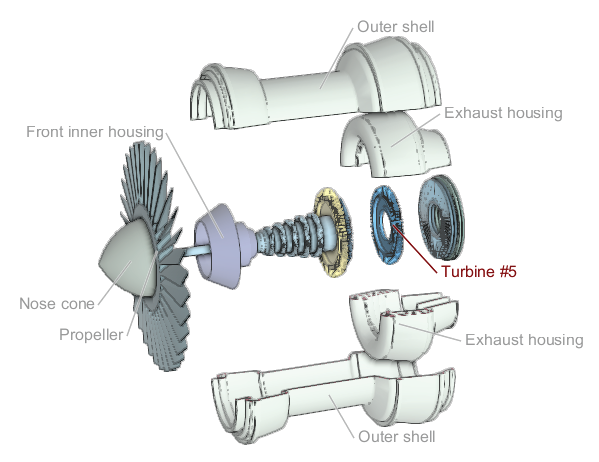
\includegraphics[height=125.0px]{img/exview3D-SIG08_1}
\end{center}
\end{frame}



\begin{frame}\frametitle{\emph{Automated generation of interactive 3D exploded view diagrams} \cite{1360700}} 
\begin{itemize}
	\item Os autores apresentam as seguintes considera��es para se criar uma vista explodida:
	\begin{itemize}
		\item \textbf{Bloqueios}:  as partes devem ser explodidas em dire��es n�o bloqueadas.
		\item \textbf{Visiblidade}: a dist�ncia entre as partes deve ser escolhida de modo que todas as partes de interesse estejam vis�veis.
		\item \textbf{Compacidade (\emph{compactness})}: a dist�ncia entre a posi��o da parte explodida e sua posi��o original deve ser minimizada.
		\item \textbf{Dire��es da explos�o}: as partes devem ser explodidas em um n�mero restrito de dire��es, facilitando a interpreta��o pelo usu�rio.
		\item \textbf{Hierarquia das partes}: partes podem ser agrupadas em cole��es.
	\end{itemize}
\end{itemize}
\end{frame}


\begin{frame}\frametitle{\emph{Automated generation of interactive 3D exploded view diagrams} \cite{1360700}} 
\begin{itemize}
	\item O algoritmo proposto pelos autores tem como entrada um modelo 3D em que as partes s�o representadas como objetos geom�tricos separados.
	\item O modelo � ent�o organizado em um grafo ac�clico dirigido:
	\begin{center}
		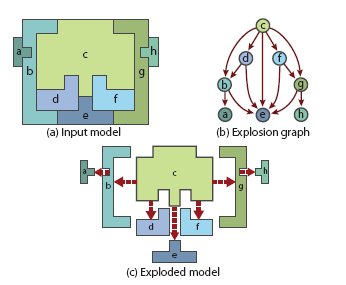
\includegraphics[height=125.0px]{img/exview3D-SIG08_2}
	\end{center}
\end{itemize}
\end{frame}

\begin{frame}\frametitle{\emph{Automated generation of interactive 3D exploded view diagrams} \cite{1360700}} 
\begin{itemize}
	\item Construindo o grafo explodido (\cite{882352}):
	\item S: conjunto com as partes ativas do modelo (ou seja, ainda n�o inseridas no grafo).
	\item P: sub-conjunto de S de partes que n�o possuam restri��o em pelo menos uma dire��o.
	\begin{enumerate}
		\item Determina P.
		\item Para cada parte $\emph{p} \in P$: determina a dist�ncia m�nima que \emph{p} teria que mover para sair do \emph{bounding box} das partes em contato com \emph{p}.
		\item \emph{p} com a menor dist�ncia � adicionado ao grafo. Arestas s�o adicionadas ligando \emph{p} a todas as outras partes que est�o em contato.
	\end{enumerate}
\end{itemize}
\end{frame}